% !Mode:: "TeX:UTF-8"

\chapter[基于图神经网络的语义依存图应用]{基于图神经网络的语义依存图应用}[Semantic Dependency Graph Application Based on Graph Neural Networks]

\section{引言}[Introduction]

\section{背景与相关工作}[Related Work]

\begin{figure}[hbtp]
	\centering
	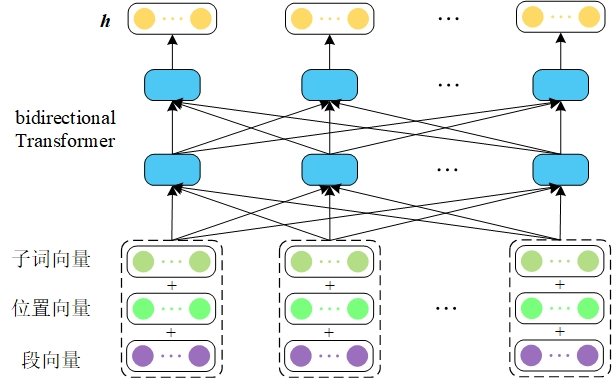
\includegraphics[width=90mm]{figures/bert.jpg}
	\caption{BERT网络结构示意图}
	\label{fig:bert}
\end{figure}

近年来以BERT\cite{devlin2019bert}为代表的在大规模无标注语料上预训练的语言模型在自然语言处理领域的众多任务上取得了很好的成绩。
BERT的训练目标为掩码语言模型(masked language modeling,MLM),即用上下文预测被遮盖(mask)的词。其神经网络结构如图~\ref{fig:bert}所示。
输入由子词(sub-word)向量、位置向量和段向量三部分相加组成。
其核心部分的双向transformer的每一层由一个多头自注意力层(multi-head self-attention layer)和一个全连接前馈层(feed-forward layer)组成。
具体来说,自注意力层计算公式为:
\begin{equation}
\label{eq:att-sum}
\mathbf{h}_i^l = \sum_{j=1}^{N} \alpha_{ij}\mathbf{W}_V \mathbf{h}_j^{l-1}
\end{equation}

\begin{equation}
\label{eq:att-weight}
\alpha_{ij} = \frac{\exp((\mathbf{W}_K \mathbf{h}_j^{l-1})^\top\mathbf{W}_Q \mathbf{h}_i^{l-1})}{\sum_{k=1}^{N}\exp((\mathbf{W}_K \mathbf{h}_k^{l-1})^\top\mathbf{W}_Q \mathbf{h}_i^{l-1})}
\end{equation}

其中$\mathbf{h}_i^l$为第$i$个词在第$l$层的隐层状态向量,$\mathbf{W}_Q$、$\mathbf{W}_K$和$\mathbf{W}_V$为模型参数矩阵。
每个多头自注意力层由$H$个上述自注意力模块组成,最后$H$个模块的隐层状态向量拼接起来作为本层的最终隐层状态向量。

为了将语义依存图中的深层语义信息融入上述预训练语言模型中,我们对自注意力模块进行如下修改:
\begin{equation}
	\label{eq:att-gat-arc}
	\mathbf{h}_{arc(i)}^l = \sum_{j\in \mathcal{N}_i} \mathbf{A}_{ij}\mathbf{W}_V \mathbf{h}_j^{l-1}
\end{equation}

其中$\mathbf{A}$为当前句子的语义依存图的邻接矩阵,$\mathcal{N}_i$表示词$i$在依存图中的相邻节点。
此外,由于句中词之间的关系(依存标签)中也包含有很重要的语义信息,我们使用一个额外模块将依存图中的依存标签信息也融入预训练语言模型中:

\begin{equation}
	\label{eq:att-gat-rel}
	\mathbf{h}_{rel(i)}^l = \sum_{j\in \mathcal{N}_i} \beta_{ij}\mathbf{W}_R \mathbf{h}_j^{l-1}
\end{equation}

\begin{equation}
	\label{eq:att-gat-rel-weight}
	\beta_{ij} = \frac{\exp(\sigma(\mathbf{W}_r \mathbf{r}_{ij} + \mathbf{b}_r))}{\sum_{k\in\mathcal{N}_i}\exp(\sigma(\mathbf{W}_r \mathbf{r}_{ij} + \mathbf{b}_r))}
\end{equation}

其中$\mathbf{r}_{ij}$为词$i$和词$j$之间的依存标签向量,$\sigma$表示激活函数。
最终将包含结构信息和标签信息的隐层向量拼接起来作为本层输出$\mathbf{h}_i^l)=[\mathbf{h}_{arc(i)}^l;\mathbf{h}_{rel(i)}^l]$。

\begin{figure}[hbtp]
	\centering
	\vspace{-1em}
	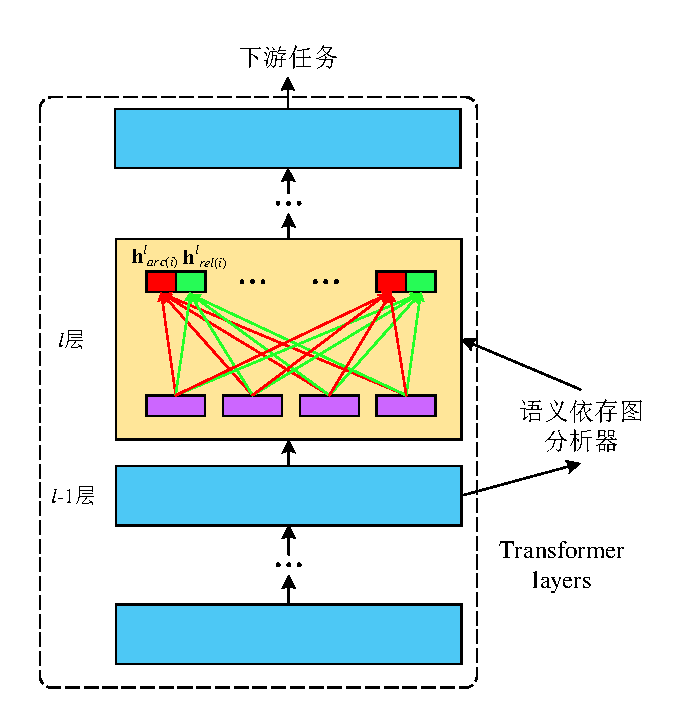
\includegraphics[width=90mm]{figures/att-gat.pdf}
	\vspace{-1.5em}
	\caption{BERT网络结构示意图}
	\label{fig:att-gat}
\end{figure}

包含语义信息的预训练语言模型结构如图~\ref{fig:att-gat}所示。
我们将BERT中的第$l$层替换为上述模块,并用第$l-1$层的输出作为依存图分析器的输入。
在训练阶段,首先用预训练好的BERT初始化参数,使用微调(fine-tuning)的方式训练依存图分析器。
之后将包含语义信息的预训练语言模型的输出作为目标任务的输入,用微调的方式同时训练目标任务和依存分析器。这部分工作正在进行中。


\section{基于字级别依存关系的预训练语言模型增强方法}[Pre-trained Model Enhancement Based on Character-Level Dependency Relations]


\section{依存关系增强的预训练语言模型的应用}[Application of Relation-Enhanced Pre-trained Models]

\subsection{基于预训练语言模型的命名实体识别模型}[Semantic Role Labeling Model Based on Pre-trained Models]

\subsection{基于预训练语言模型的关系抽取模型}[Relation Extraction Model Based on Pre-trained Models]


\section{实验与分析}[Experiments and Analysis]

\subsection{实验设置}[Experimental Settings]


\section{本章小结}[Conclusions]


% Local Variables:
% TeX-master: "../thesis"
% TeX-engine: xetex
% End: